\section{Design of the Chorus and Flanger Effect}\label{chor_des}

\subsection{Obtaining the Differential Equation}

The flanger- and chorus- effect are similar in their design so they will be presented in the same section. \\

From the block diagram presented in section \autoref{sec:chorus}, a block diagram in the discrete time domain for the flanger and chorus effect can be obtained and is shown in \autoref{fig:chorus_diag_des}. \\ 
The chorus effect is the one in red and black while the flanger is only in black.  
\begin{figure} [htbp!]
	\centering
\begin{picture}(0,0)%
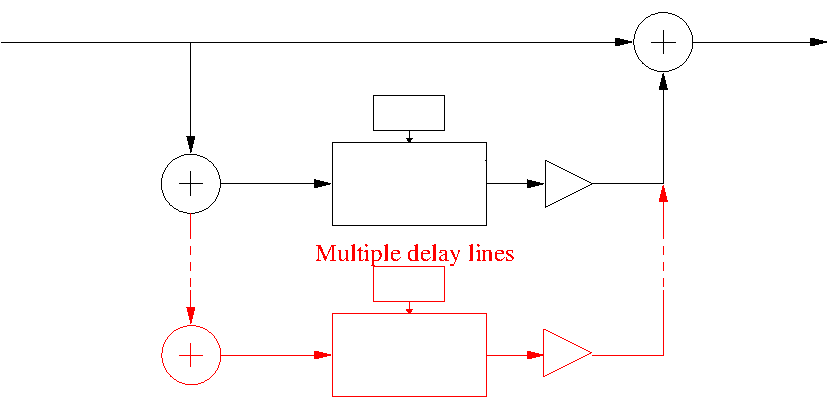
\includegraphics{chorus_diag_des.pdf}%
\end{picture}%
\setlength{\unitlength}{4144sp}%
%
\begingroup\makeatletter\ifx\SetFigFont\undefined%
\gdef\SetFigFont#1#2#3#4#5{%
	\reset@font\fontsize{#1}{#2pt}%
	\fontfamily{#3}\fontseries{#4}\fontshape{#5}%
	\selectfont}%
\fi\endgroup%
\begin{picture}(6327,3018)(3766,-3493)
\put(6571,-1906){\color[rgb]{0,0,0}$z^{-d_{1}}$}%

\put(8101,-1636){\color[rgb]{0,0,0}$g_{1}$}%

\put(6616,-3211){\color[rgb]{1,0,0}$z^{-d_{2}}$}%

\put(8101,-2986){\color[rgb]{1,0,0}$g_{2}$}%

\put(6706,-2671){\color[rgb]{1,0,0}\textit{LFO}}%

\put(6706,-1366){\color[rgb]{0,0,0}\textit{LFO}}%

\put(3781,-646){\color[rgb]{0,0,0}\textit{x[n]}}%

\put(9406,-646){\color[rgb]{0,0,0}\textit{y[n]}}%

\end{picture}%
\caption{Block Diagram of the chorus and flanger effect in the discrete time domain.}
\label{fig:chorus_diag_des}
\end{figure}

From \autoref{fig:chorus_diag_des}, the following differential equations can be inferred:

The equation for the flanger can be written as in \autoref{eq:flang_eq}
\begin{equation}
\label{eq:flang_eq}
		y[n] = x[n] + x[n- d_{1}] \cdot g_{1}  
\end{equation}

The equation for the chorus can be written as in \autoref{eq:chor_eq}:

\begin{equation}
\label{eq:chor_eq}
y[n] = x[n] + \sum_{j=1}^{i}  (x[n- d_{j}] \cdot g_{j})
\end{equation}

The index $i$ represents the number of delays that are being implemented in the chorus effect which is also the chorus size. Index $n$ represents the present sample. \\
If the implementation is done using a time varying delay, equations \ref{flang_eq} and \ref{chor_eq} can be re-written as \autoref{eq:flang_eq2} and \autoref{eq:chor_eq2}:

\begin{equation}
\label{eq:flang_eq2}
y[n] = x[n] + x[n- d_{1}[n]] \cdot g_{1}  
\end{equation}

\begin{equation}
\label{eq:chor_eq2}
y[n] = x[n] + \sum_{j=1}^{i}  (x[n- d_{j}[n]] \cdot g_{j})
\end{equation}

The delay value has to be a periodic function that is varying in a user-defined range. As illustrated in \autoref{fig:chorus_diag_des}, this varying delay can be made from a \gls{lfo}.

The LFO that makes the delay vary is a sine wave in the chorus and the flanger effect. In the case of the flanger, the user can set the LFO frequency between 0,1 and 10 Hz and only the boundaries for the chorus. 
The gain for the flanger effect can be chosen by the user. For the chorus, the user can choose the boundaries of the gain value that will be randomly selected for each of the delay lines. 
The number of delay lines for the chorus effect is also a choice but should not exceed 4, the reason is that after 4 lines it has been found that the effect has a strange sound. 
The delay time for the flanging effect should be between 1 and \SI{20}{\milli\second} while the delay time in the chorus should be longer than \SI{20}{\milli\second}. 

A delay can be done in different ways digitally. One way is to use a ring buffer also known as circular buffer. \\
The idea of this data structure is that it takes values and only outputs them when it gets full, and overwrites the oldest after outputting it. It is a kind of a FIFO queue structure but where the start and the overwriting can start at any index. \\
This means that the size of the buffer depends on the delay.  The buffer size must then be always up-to-date with the new delay value. \\ 
The value of the delay is determined by a periodic function as said before, different waveforms can be used as said in \autoref{chor_flang}. A common periodic function that can be used is the sine. Since it varies between 0 and 1, it can be then multiplied with the user-defined range. 
The delay can then be written as in \autoref{eq:sine_delay}.

\begin{equation}\label{eq:sine_delay}
	d[n]= A \cdot sin(2\pi  \cdot \frac{f_{l}}{f_{s}} n)
\end{equation}

\startexplain
     \explain{$A$ is the value of the user-defined range which is also the depth.}{\si{1}}
     \explain{$f_{s}$ the sampling frequency.}{\si{\hertz}}
     \explain{$f_{l}$ is the frequency of the \gls{lfo}.}{\si{\hertz}}
    \stopexplain 

\subsection{Making the LFO by Cordic algorithm}
The \gls{lfo} in both the chorus- and the flanger- effect should, as stated in \autoref{chor_des}, be able to make sine waves from \SI{0.1}{\kilo\hertz} to \SI{10}{\kilo\hertz}. A \gls{dsp} is not necessarily able to calculate sine values and therefore an algorithm has to be implemented in order to make this possible. A way to do this is by using the \gls{cordic} algorithm, which can be used to calculate both sine, cosine, square roots etc \citep{cordic}. 
When using the \gls{cordic} algorithm for for an \gls{lfo} the two equations \autoref{eq:cordic_x} and \autoref{eq:cordic_y} are almost all what is needed.

\begin{equation}
\label{eq:cordic_x}
		x_{n+1} = x_n \cdot \cos(\theta) - y_n \cdot \sin(\theta) 
\end{equation}
\startexplain
     \explain{$x_{n+1}$ is the present cosine value.}{\si{1}}
     \explain{$x_n$ is the previous cosine value.}{\si{1}}
     \explain{$y_n$ is the previous sine value.}{\si{1}}
     \explain{$yn$ is the index.}{\si{1}}
    \stopexplain 

\begin{equation}
\label{eq:cordic_y}
		y_{n+1} = y_n \cdot \cos(\theta) + x_n \cdot \sin(\theta) 
\end{equation}
\startexplain
     \explain{$y_{n+1}$ is the present sine value.}{\si{1}}
\stopexplain

The algorithm works by initializing $x_0$ to 1 and $y_0$ to 0. This way $x_1$ becomes equal to $\cos(\theta)$ and $y_1$ becomes equal to $\sin(\theta)$. When the next iteration begins, the initial vector will then have the coordinates [$x_1$, $y_1$]. This way $x_2$ becomes equal to $\cos(2 \cdot \theta)$ and $y_2$ becomes equal to $\sin(2 \cdot \theta)$. Thus it is only necessary to calculate $\cos(\theta)$ and $\sin(\theta)$ and then follow the iterations to produce a sine wave. The frequency of the sine wave is decided by $\theta$. The relation between the frequency and $\theta$ is shown in \autoref{eq:cordic_freq}.

\begin{equation}
\label{eq:cordic_freq}
		\theta = 2 \cdot \pi \cdot \frac{f}{f_s} 
\end{equation}
\startexplain
     \explain{$f$ is the wanted frequency of the sine wave.}{\si{\hertz}}
     \explain{$f_s$ is the sampling frequency.}{\si{\hertz}}
\stopexplain 

This way the \gls{cordic} algorithm will have $\frac{f_s}{f}$ steps round the unitcircle and thereby produce a sine wave with frequency $f$ and sine values between $\pm$1.
A MATLAB simulation of the \gls{cordic} algorithm was made and set to produce a \SI{1}{\hertz} sine wave. The result of the simulation is shown in \autoref{fig:cordic_1Hz}.

\begin{figure}[!h]
    \centering
        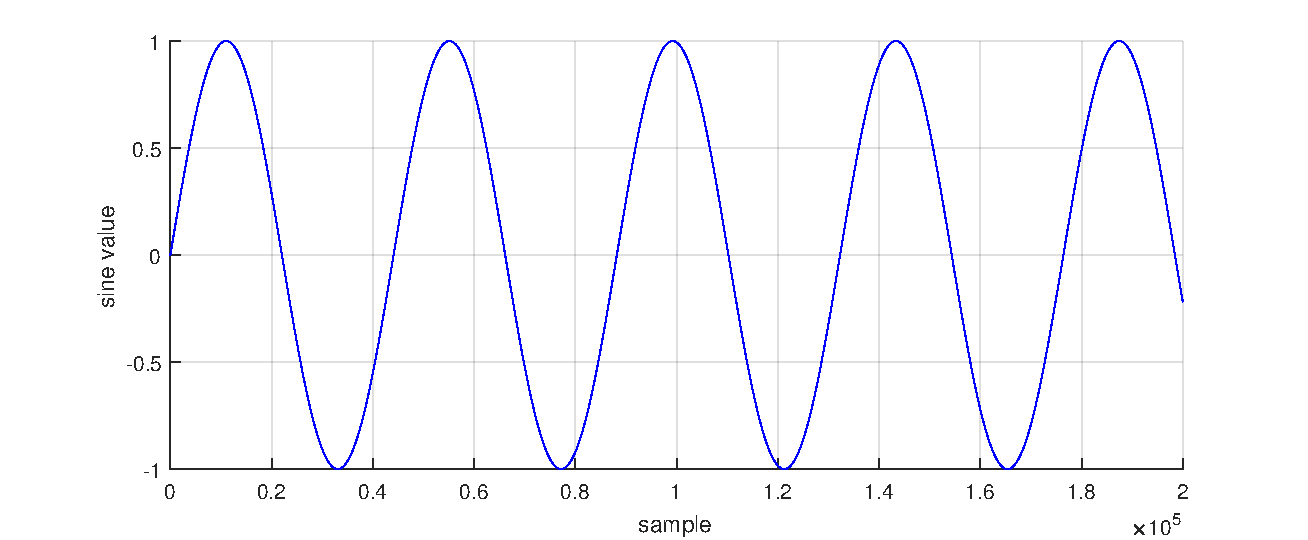
\includegraphics[width=\textwidth]{cordic_1Hz.pdf}
        \caption{Simulation of the \gls{cordic} algorithm, set to produce a \SI{1}{\hertz} sine wave.}
        \label{fig:cordic_1Hz}
  \end{figure}
  
When implementing the \gls{cordic} algorithm on a \gls{dsp}, the calculated $\cos(\theta)$ and $\sin(\theta)$ values in \autoref{eq:cordic_x} and \autoref{eq:cordic_y}, might have to be changed a bit to make the algorithm stable. 

\subsection{Implementation of the CORDIC algorithm}
When implementing the CORDIC algorithm on the \gls{dsp}, some choices have to be made to begin with. The first choice is the resolution of the calculations. Because the \gls{lfo} has to produce such low frequencies, it is chosen to work in 32-bit precision. Since all the values in the CORDIC calculations are between $\pm$ 1, it is chosen to divide the 32-bits into one sign bit, one integer bit and 30 fraction bits, which should make the CORDIC algorithm able to produce a \SI{0.4}{\hertz}.
It is mainly the two equations \autoref{eq:cordic_x} and \autoref{eq:cordic_y} that has to be implemented. Because it is chosen to operate in 32-bits precision all calculations have to be made twice. Multiplication is e.g. done by the following algorithm:
\begin{itemize}
\item The two variables $a$ and $b$ both have a high (16-bits) and a low part (16-bits).
\item At first the low part of $a$ is multiplied with high part of $b$ and saved in $c_{LH}$.
\item Then the low part of $a$ is multiplied with the low part of $b$ and saved in $c_{LL}$.
\item $c_{LH}$ and $c_{LL}$ are then added in $d_L$ which is a 32-bit value containing [$c_{LH}$ $c_{LL}$].
\item Afterwords the high part of $a$ is multiplied with the high part of $b$ and saved in $c_{HH}$.
\item Then the high part of $a$ is multiplied with the low part of $b$ and saved in $c_{HL}$.
\item $c_{HH}$ and $c_{HL}$ are then added in $d_H$ which is a 32-bit value containing [$c_{HH}$ $c_{HL}$].
\item The final result of the multiplication is then found by shifting $d_L$ to a 16-bit value and add it to the 32-bit value $d_H$.
\end{itemize}

An example of this in the \gls{cordic} algorithm is in \autoref{code:cordic_2} where the 32-bit value $x_n$ is multiplied with the 32-bit value $\cos(\theta)$.
\includeCode{cordic_2.asm}{assembly}{19}{59}{Multiplying $x_n$ with $\cos(\theta)$ in the CORDIC algorithm}{code:cordic_2}{code/design/}

\subsection{Approximation of Values Lying between Two Samples}

In some cases during the chorus and the flanger effect, the delay value require an approximation between two of the delayed samples in the buffer. It happens when the delay is between two samples and not at an exact sample. In order to solve this problem, a linear approximation between the two samples has to be made. \\

Here is an illustration in the figure \ref{fig:signal_approx} of the distances and segments that are involved in the approximation. \\



\begin{figure}[htbp]
	\centering
	\begin{picture}(0,0)%
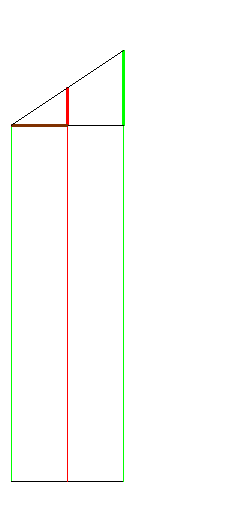
\includegraphics{flang_approx.pdf}%
\end{picture}%
\setlength{\unitlength}{3947sp}%
%
\begingroup\makeatletter\ifx\SetFigFont\undefined%
\gdef\SetFigFont#1#2#3#4#5{%
  \reset@font\fontsize{#1}{#2pt}%
  \fontfamily{#3}\fontseries{#4}\fontshape{#5}%
  \selectfont}%
\fi\endgroup%
\begin{picture}(1874,4161)(4261,-4876)
\put(5251,-886){\makebox(0,0)[lb]{\smash{{\SetFigFont{12}{14.4}{\rmdefault}{\mddefault}{\updefault}{\color[rgb]{0,0,0}$Y_{2}$}%
}}}}
\put(5551,-1411){\makebox(0,0)[lb]{\smash{{\SetFigFont{12}{14.4}{\rmdefault}{\mddefault}{\updefault}{\color[rgb]{0,0,0} $\Delta Y$}%
}}}}
\put(4351,-1936){\makebox(0,0)[lb]{\smash{{\SetFigFont{12}{14.4}{\rmdefault}{\mddefault}{\updefault}{\color[rgb]{0,0,0} $\Delta X$}%
}}}}
\put(4876,-1561){\makebox(0,0)[lb]{\smash{{\SetFigFont{12}{14.4}{\rmdefault}{\mddefault}{\updefault}{\color[rgb]{0,0,0}$Y'$}%
}}}}
\put(4351,-4861){\makebox(0,0)[lb]{\smash{{\SetFigFont{12}{14.4}{\rmdefault}{\mddefault}{\updefault}{\color[rgb]{0,0,0}$X_{1}$}%
}}}}
\put(5251,-4786){\makebox(0,0)[lb]{\smash{{\SetFigFont{12}{14.4}{\rmdefault}{\mddefault}{\updefault}{\color[rgb]{0,0,0}$X_{2}$}%
}}}}
\put(4276,-1561){\makebox(0,0)[lb]{\smash{{\SetFigFont{12}{14.4}{\rmdefault}{\mddefault}{\updefault}{\color[rgb]{0,0,0}$Y_{1}$}%
}}}}
\end{picture}%
\caption{Linear approximation of the signal}
	\label{fig:signal_approx}
\end{figure}

The goal is to determine the length of red line. The red line is the sum of $Y_{1}$ and $Y'$. $Y_{1}$ is known and $Y'$ is the unknown length to be determined by calculations. \\

The equation is:

\begin{equation}
	Y' = \Delta X - (\Delta X \cdot \Delta Y)
\end{equation}

$\Delta Y$ is determined by doing the difference between $Y_{1}$ and $Y_{2}$. 

\subsection{Memory Mapping for the Chorus and the Flanger Effect Coefficients and Data}


Here is the memory mapping for the chorus and flanger effect in figure \ref{fig:memory_map_chor}.

\begin{figure}[htbp]
	\centering

\begin{picture}(0,0)%
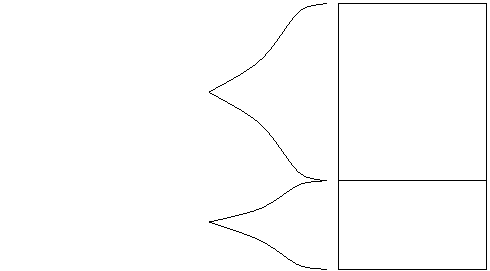
\includegraphics{Flang_chor_mem.pdf}%
\end{picture}%
\setlength{\unitlength}{4144sp}%
%
\begingroup\makeatletter\ifx\SetFigFont\undefined%
\gdef\SetFigFont#1#2#3#4#5{%
  \reset@font\fontsize{#1}{#2pt}%
  \fontfamily{#3}\fontseries{#4}\fontshape{#5}%
  \selectfont}%
\fi\endgroup%
\begin{picture}(3312,1419)(9076,-4798)
\put(11476,-4696){\makebox(0,0)[lb]{\smash{{\SetFigFont{12}{14.4}{\rmdefault}{\mddefault}{\updefault}{\color[rgb]{0,0,0}0x46EA}%
}}}}
\put(9136,-4516){\makebox(0,0)[lb]{\smash{{\SetFigFont{12}{14.4}{\rmdefault}{\mddefault}{\updefault}{\color[rgb]{0,0,0}Coefficients}%
}}}}
\put(9091,-3796){\makebox(0,0)[lb]{\smash{{\SetFigFont{12}{14.4}{\rmdefault}{\mddefault}{\updefault}{\color[rgb]{0,0,0}Delay Buffer}%
}}}}
\put(11476,-3661){\makebox(0,0)[lb]{\smash{{\SetFigFont{12}{14.4}{\rmdefault}{\mddefault}{\updefault}{\color[rgb]{0,0,0}0x3FCB}%
}}}}
\put(11476,-4021){\makebox(0,0)[lb]{\smash{{\SetFigFont{12}{14.4}{\rmdefault}{\mddefault}{\updefault}{\color[rgb]{0,0,0}0x46D9}%
}}}}
\put(11476,-4336){\makebox(0,0)[lb]{\smash{{\SetFigFont{12}{14.4}{\rmdefault}{\mddefault}{\updefault}{\color[rgb]{0,0,0}0x46DA}%
}}}}
\end{picture}%


\caption{Memory Mapping for the Chorus and the Flanger Effects}
	\label{fig:memory_map_chor}
\end{figure}



